\chapter*{Závěr}

Cílem této práce bylo navrhnout ucelený systém, který dokáže:

\begin{itemize}
    \item automaticky počítat upletené ponožky
    \item on-line hlásit poruchu na stroji a~zjišťovat celkovou poruchovost strojů
    \item porovnávat výkonnost jednotlivých pracovních směn
    \item monitorovat průběh výroby
    \item nahradí část monotónní práce operátora
    \item zrychlí a~zefektivní výrobu
    \item sníží chybovost
\end{itemize}

Všechny tyto vytyčené cíle se mi podařilo splnit. Systém nadále běží ve firmě ROTEX Vysočina s.r.o~\cite{ROTEX} a~pomáhá v~běžném provozu.
Můj systém se stal nedílnou součástí výrobního procesu a analyzuje a~zefektivňuje průběh výroby.

Systém je k 1. únoru 2021 nasazen na deseti pletacích strojích a po dobu provozu zaznamenal již přes padesát tisíc upletených ponožek bez závady na senzorech.
% Celý systém je nasazený krátkou dobu, abych dokázal porovnat produktivitu před nasazením tohoto systému s~daty po nasazení.

Velkým přínosem pro firmu je porovnávání pracovních směn, díky kterým zaměstnavatel ihned vidí rozdíly mezi produktivitou práce v~daném čase.

Díky SOČ jsem se naučil navrhovat plošné spoje, rozšířil jsem si obzory v~elektronice a~při vývoji jsem si vyzkoušel práci s~měřícími přístroji. 
Také jsem se naučil programovat v~jazyce PHP a~vytvářet komplexní webové systémy.

V~budoucnu bych chtěl tento systém rozšířit na všechny pletací stroje a~pokrýt tak celou výrobu.
Taktéž pokračuji na vylepšování webové aplikace a~plánuji ji rozšířit o~další funkce.
Jde například o~export dat do tabulek.

Tuto práci můžete najít na adrese: \url{https://github.com/JakubAndrysek/SOC-Integrace-do-prumyslu-4.0/blob/master/text.pdf}.

Všechny zdrojové kódy a~DPS k~projektu jsou k~dispozici na \url{https://github.com/Pletacka-IoT} pod MIT licencí.

\begin{figure}[htbp]
    \centering
    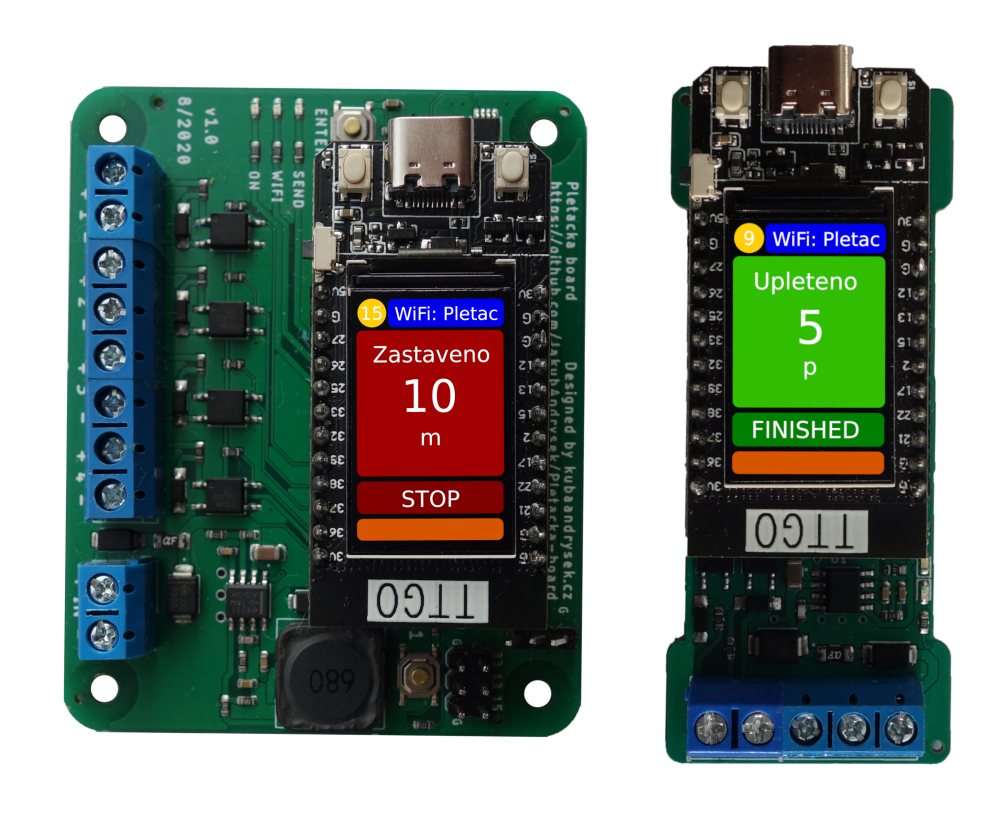
\includegraphics[width=\textwidth]{img/Oba.png}
    \caption{Senzory}
    \label{fig:senzory}
\end{figure}


\newpage